\section{eo\-Persistent Class Reference}
\label{classeo_persistent}\index{eoPersistent@{eoPersistent}}
An persistent object that knows how to write (through functions inherited from {\bf eo\-Printable}{\rm (p.\,\pageref{classeo_printable})}\#) and read itself.  


{\tt \#include $<$eo\-Persistent.h$>$}

Inheritance diagram for eo\-Persistent::\begin{figure}[H]
\begin{center}
\leavevmode
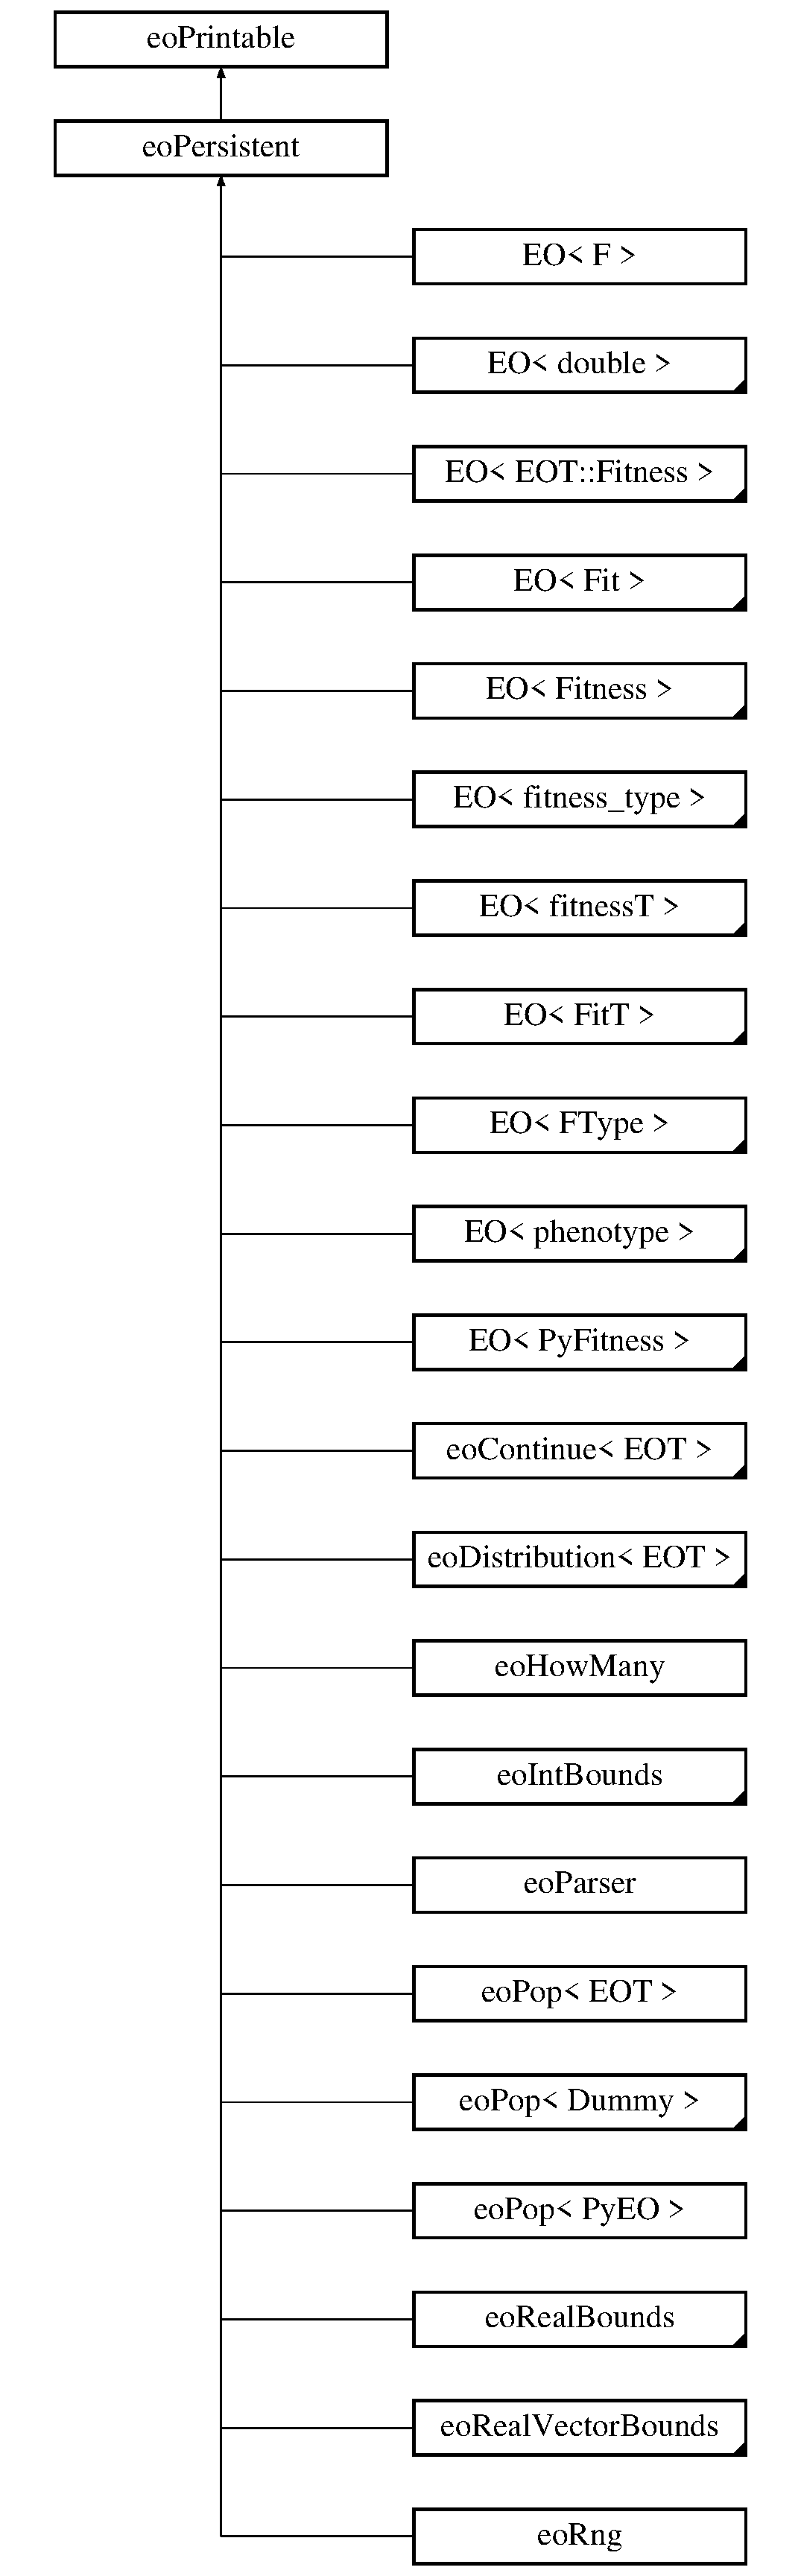
\includegraphics[height=12cm]{classeo_persistent}
\end{center}
\end{figure}
\subsection*{Public Member Functions}
\begin{CompactItemize}
\item 
virtual {\bf $\sim$eo\-Persistent} ()\label{classeo_persistent_a0}

\begin{CompactList}\small\item\em Virtual dtor. They are needed in virtual class hierarchies. \item\end{CompactList}\item 
virtual void {\bf read\-From} (std::istream \&\_\-is)=0
\begin{CompactList}\small\item\em Read object. \item\end{CompactList}\end{CompactItemize}


\subsection{Detailed Description}
An persistent object that knows how to write (through functions inherited from {\bf eo\-Printable}{\rm (p.\,\pageref{classeo_printable})}\#) and read itself. 



Definition at line 52 of file eo\-Persistent.h.

\subsection{Member Function Documentation}
\index{eoPersistent@{eo\-Persistent}!readFrom@{readFrom}}
\index{readFrom@{readFrom}!eoPersistent@{eo\-Persistent}}
\subsubsection{\setlength{\rightskip}{0pt plus 5cm}virtual void eo\-Persistent::read\-From (std::istream \& {\em \_\-is})\hspace{0.3cm}{\tt  [pure virtual]}}\label{classeo_persistent_a1}


Read object. 

\begin{Desc}
\item[Parameters:]
\begin{description}
\item[{\em \_\-is}]A std::istream. \end{description}
\end{Desc}
\begin{Desc}
\item[Exceptions:]
\begin{description}
\item[{\em runtime\_\-std::exception}]If a valid object can't be read. \end{description}
\end{Desc}


Implemented in {\bf EO$<$ F $>$} {\rm (p.\,\pageref{class_e_o_z10_1})}, {\bf eo\-Continue$<$ EOT $>$} {\rm (p.\,\pageref{classeo_continue_a1})}, {\bf eo\-Gen\-Continue$<$ EOT $>$} {\rm (p.\,\pageref{classeo_gen_continue_a6})}, {\bf eo\-Pop$<$ EOT $>$} {\rm (p.\,\pageref{classeo_pop_z19_0})}, {\bf eo\-Vector$<$ Fit\-T, Gene\-Type $>$} {\rm (p.\,\pageref{classeo_vector_a5})}, {\bf eo\-Es\-Full$<$ Fit $>$} {\rm (p.\,\pageref{classeo_es_full_a3})}, {\bf eo\-Es\-Simple$<$ Fit $>$} {\rm (p.\,\pageref{classeo_es_simple_a3})}, {\bf eo\-Es\-Stdev$<$ Fit $>$} {\rm (p.\,\pageref{classeo_es_stdev_a3})}, {\bf eo\-Bit$<$ Fit\-T $>$} {\rm (p.\,\pageref{classeo_bit_a3})}, {\bf eo\-PBILDistrib$<$ EOT $>$} {\rm (p.\,\pageref{classeo_p_b_i_l_distrib_a4})}, {\bf eo\-Parse\-Tree$<$ FType, Node $>$} {\rm (p.\,\pageref{classeo_parse_tree_a6})}, {\bf eo\-External\-EO$<$ Fit, External $>$} {\rm (p.\,\pageref{classeo_external_e_o_a3})}, {\bf eo\-How\-Many} {\rm (p.\,\pageref{classeo_how_many_a6})}, {\bf eo\-Int\-No\-Bounds} {\rm (p.\,\pageref{classeo_int_no_bounds_a13})}, {\bf eo\-Int\-Interval} {\rm (p.\,\pageref{classeo_int_interval_a14})}, {\bf eo\-Int\-Below\-Bound} {\rm (p.\,\pageref{classeo_int_below_bound_a14})}, {\bf eo\-Int\-Above\-Bound} {\rm (p.\,\pageref{classeo_int_above_bound_a14})}, {\bf eo\-General\-Int\-Bounds} {\rm (p.\,\pageref{classeo_general_int_bounds_a19})}, {\bf eo\-Parser} {\rm (p.\,\pageref{classeo_parser_a2})}, {\bf eo\-Real\-No\-Bounds} {\rm (p.\,\pageref{classeo_real_no_bounds_a12})}, {\bf eo\-Real\-Interval} {\rm (p.\,\pageref{classeo_real_interval_a13})}, {\bf eo\-Real\-Below\-Bound} {\rm (p.\,\pageref{classeo_real_below_bound_a13})}, {\bf eo\-Real\-Above\-Bound} {\rm (p.\,\pageref{classeo_real_above_bound_a13})}, {\bf eo\-General\-Real\-Bounds} {\rm (p.\,\pageref{classeo_general_real_bounds_a18})}, {\bf eo\-Real\-Vector\-Bounds} {\rm (p.\,\pageref{classeo_real_vector_bounds_a7})}, {\bf eo\-Rng} {\rm (p.\,\pageref{classeo_rng_a17})}, {\bf EO$<$ double $>$} {\rm (p.\,\pageref{class_e_o_z10_1})}, {\bf EO$<$ EOT::Fitness $>$} {\rm (p.\,\pageref{class_e_o_z10_1})}, {\bf EO$<$ Fit\-T $>$} {\rm (p.\,\pageref{class_e_o_z10_1})}, {\bf EO$<$ phenotype $>$} {\rm (p.\,\pageref{class_e_o_z10_1})}, {\bf EO$<$ fitness\-T $>$} {\rm (p.\,\pageref{class_e_o_z10_1})}, {\bf EO$<$ Fit $>$} {\rm (p.\,\pageref{class_e_o_z10_1})}, {\bf EO$<$ FType $>$} {\rm (p.\,\pageref{class_e_o_z10_1})}, {\bf EO$<$ fitness\_\-type $>$} {\rm (p.\,\pageref{class_e_o_z10_1})}, {\bf EO$<$ Fitness $>$} {\rm (p.\,\pageref{class_e_o_z10_1})}, {\bf EO$<$ Py\-Fitness $>$} {\rm (p.\,\pageref{class_e_o_z10_1})}, {\bf eo\-Pop$<$ Py\-EO $>$} {\rm (p.\,\pageref{classeo_pop_z19_0})}, {\bf eo\-Pop$<$ Dummy $>$} {\rm (p.\,\pageref{classeo_pop_z19_0})}, {\bf eo\-Vector$<$ Fit, double $>$} {\rm (p.\,\pageref{classeo_vector_a5})}, {\bf eo\-Vector$<$ Fit\-T, double $>$} {\rm (p.\,\pageref{classeo_vector_a5})}, and {\bf eo\-Vector$<$ Fit\-T, bool $>$} {\rm (p.\,\pageref{classeo_vector_a5})}.

Referenced by eo\-State::load().

The documentation for this class was generated from the following file:\begin{CompactItemize}
\item 
eo\-Persistent.h\end{CompactItemize}
